% AOSD report template
% Jakub Perdek 2020

%\documentclass[11pt,english,a4paper,twoside]{article}
\documentclass[11pt,slovak,a4paper,twoside]{article}



\usepackage[slovak]{babel}
\usepackage[utf8]{inputenc}
\usepackage[T1]{fontenc}

\usepackage{url}
\usepackage[nottoc]{tocbibind}
\usepackage{ifthen}
\usepackage{float}
\usepackage[hidelinks]{hyperref}
\usepackage{graphicx}
\usepackage{listings}


\newcommand{\magnf}{.65}
\newcommand{\codesize}{\footnotesize}
\newcommand{\lsti}{\ajset\lstinline[basicstyle=\fontsize{10}{12}\selectfont]}
\newcommand{\emp}[1]{\emph{#1}}
\newcommand{\ffe}[1]{\textsf{#1}}

% balík listings niekedy niektoré kľúčové slová nezvýrazňuje ak to nedostane príkazom tesne pred textom
\newcommand{\ajset}{\lstset{emph={class,aspect,new,call,execution,set,int,advice,public,thisJoinPointStaticPart,thisEnclosingJoinPointStaticPart,@annotation,dominates},emphstyle=\bfseries}}

\newcommand{\reporttitle}{Aspect oriented configuration of software product line features} % here goes your fancy title

\pagestyle{myheadings}
\markboth{\reporttitle}{Quality of refactored code, modularity and product derivation 2021/22, FIIT STU}

\title{\reporttitle}

\author{Jakub Perdek} % your name

\date{In\v{s}titút informatiky, informa\v{c}ných systémov a softvérového in\v{z}inierstva\\
      Fakulta informatiky a informa\v{c}ných technológií\\
      Slovenská technická univerzita v Bratislave\\[6pt]
      20. Október, 2021} % modify the date if different



\begin{document}

\maketitle

\begin{abstract}
Generovanie variantov produktov pomáha vytvori\v{t} produkty z danej domény efektívnej\v{s}ie a lacnej\v{s}ie. Nevzniká tak iba jeden produkt, ale \v{l}ahko adaptovate\v{l}né produkty pre rôzne prostredia, jazyky a \v{d}al\v{s}ie po\v{z}iadavky (Beuche a Dalgarno 2006). Derivova\v{t} produkty prispôsobené po\v{z}adovanej variabilite mo\v{z}no za pomoci aspektovo orientovaného prístupu, hlavne jazyka AspectJ  \cite{young_using_1999} (Young a Math, 1999), ktorého mo\v{z}nosti by sme chceli pri tejto úlohe preskúma\v{t}. Vyberáme pou\v{z}itie jazyka AspectJ, preto\v{z}e umo\v{z}\v{n}uje oddeli\v{t} zále\v{z}itosti ako je logovanie, ke\v{s}ovanie, poolovanie, ale hlavne je mo\v{z}né vyradi\v{t} z vykonávania vybrané aspekty, respektíve isté vlastnosti aplikácie, prípadne aj celkovú závislos\v{t} na tomto jazyku \cite{laddad_aspectj_2003} (Laddad, 2003).												

Zaujíma nás preto uplatnenie jazyka pri umo\v{z}není konfigurovate\v{l}nosti konkrétnych vlastností v kóde, a samotné generovanie konkrétneho variantu produktu s prípadnou po\v{z}iadavkou nezávislosti implementácie od tohto pou\v{z}itého jazyka. Zhodnotíme prínosy a kvality aspektovo orientovaného prístupu na konkrétnej implementácii, a porovnáme ich s identifikovanými problémami a benefitmi spomenutými v rôznych reimplementáciách u\v{z} existujúcich softvérových systémov ako je vedecká kalkula\v{c}ka (Botterweck, 2009) alebo databázový systém (Kastner, 2007). Samotné analýzy nazna\v{c}ujú význam vo\v{l}by domény pri zostrojovaní radu softvérových produktov, preto by sme v neposlednom rade chceli porovnať vplyv domény pri ich implementácii.								

Plánujeme prispôsobi\v{t} existujúcu hru Battleship tak, aby umo\v{z}\v{n}ovala mana\v{z}ova\v{t} vlastnosti na základe u\v{z} vytvoreného modelu vlastností, vä\v{c}\v{s}ina ktorých nie je vôbec implementovaná. Cie\v{l}om je aj analyzova\v{t} spôsoby odvodenia konkrétneho produktu, a mieru jeho závislostí od jazyka AspectJ. 								

\v{D}al\v{s}ou aplikáciou pre analýzu je odvodzovanie rôznych fraktálov (uká\v{z}ky typov nájdete v Pelánek, 2012) z pôvodného algoritmu, ktoré by sme realizovali zásahom aspektov do jeho vykonávania. Predpokladáme, \v{z}e úloha samotného návrhu vlastností pre uvedenú aplikáciu je ur\v{c}ená hodnotou vzh\v{l}adu fraktálu, pri\v{c}om zhotovenie radu produktov pre\v{n} mô\v{z}e vy\v{z}adova\v{t} iné nároky na model vlastností, ako napríklad generovanie v\v{s}etkých mo\v{z}ných derivácií pre následné overenie estetiky a identifikovanie najvhodnej\v{s}ích kandidátov. Zamý\v{s}\v{l}ame preto zhodnoti\v{t} význam prípadného potenciálu aspektovo orientovaného rie\v{s}enia pre derivovanie konkrétnych fraktálov.
\end{abstract}


\section{Introduction} \label{introduction}
Creation of software products needs to create project and develop given solution according requirements. This is often expensive and needs analysis for every such project. One possible way is to implement software product line to make possible derive such resulting products or components and evolve then on basis of domain knowledge. Some features can be too expensive for customer to pay for them and because of it they are ommited. Others collide with necessary ones and needs to be ommited too. 

Appropriate domain analysis is required to design mandatory and voluntary features of the given system to know which products should be possible to generate and if it brings value to customer and his changing requirements. For this purpose we used feature models. In reality many of these models can exist, but only few them can support these changing needs. We think that few relations in feature model can be expressed and solved by aspect and classes almost similarly for each group of them. But sometimes features can collide and some features can't be used together. Because of mentioned problem, its necessary to think about derivation of given product and developing certain feature without colliding ones.  

In our work we try to focus on applying aspect oriented language to develop program on feature model basis to serve as software product line. During our work we analyze applying ways how to do it in AspectJ language and its consequences on code quality, encapsulation, modularity benefits and dependencies which arise with using AspectJ language. We used hints and advices from papers which provided refactoring on many systems using aspect orientated languages, especially previously mentioned AspectJ.

Provided software product line and our development techniques can be later applied on fractal construction. New shapes and patterns applied at given positions during recursion drawing of given fractal are voluntary features of given model. To perceive potential aesthetic feeling from some of them is necessary to derive such products. Having appropriate product line enabling generate full range of products for their next validation is the main requirement for this specific task.

  

\section{Overview of sections} \label{content}

Section~\ref{domainAnalysis} describes software product line and domain analysis applied to its creation. Actual state and design of Battleship game is described in section~\ref{actualGameState}. Applied techniques for solution refactoring are presented in section~\ref{gameRefactoring}. In section~\ref{gameDerivation} we present a game derivation based on actual configuration settings and introducing annotations and expression which helps to choose content to copy in result project. 
Section~\ref{allDerivations} describes how is possible to create all possible derivations based on feature model of given solution. We are using Battleship game again with appropriate feature model for this purpose. 

We mentioned possible applications for deriving fractals in section~\ref{fractalProductLine}. Making the best design of software product line which enables derivation in all possible cases to enrich our perception and produce patterns for next validation is main goal here.  

In section~\ref{resultingModularity} we conclude impacts on modularity. We also analyze these impacts using aspect oriented programming and a given case of software product line approach.

Work which is done in given area is described in section~\ref{recentWork}. We describe some existing approaches solving similar problems that we have.

Our conclusions and next work we mentioned in section~\ref{conclusions}.



\section{Software product line and domain analysis} \label{domainAnalysis}


\section{Actual state and design of solution for Battleship game} \label{actualGameState}

To provide the most appropriate feature model which can capture potential needs of customer and domain knowledge to serve as basis for our later analysis we choose already provided one. Mentioned feature model is a part of the Battleship game in one repository for which depicts its features. Battleship game is simple game consisting of two players trying to destroy ships to each other. Lot of improvements are possible to include as additional features to make the game more interesting. We think that given feature model is based of performed domain analysis and identified many features with decision of their optionality.

Firstly, we need to mention some problems of provided implementation of Java Battleship game. Only some of mandatory features were provided in unconfigurable way. From feature model we can name features like player names, collecting statistics, computer strategy subtree and challenge as unimplemented. Many features are hardcoded and can not be easily enhanced without code refactoring. Other aspect of such implementation is that user cant choose one option from given options without modifying code. For example choosing difficulty option in the game. The same code is repeated in many classes and methods. It lacks of some object oriented programming practises. No encapsulation resulting in free access to public variables from any class. Another identified problem was that concerns were not fully separated. For example setup of player was not included in player class. Some static method should be converted to dynamic ones to be associated to given instance. This game use console only and not have any graphic user interface. We let console interface as is. Implementation not provide any possibility of product derivation at all. Potential refactoring was required then. 

Mentioned Battleship game is not large and not have many features, but can serve as potential board game domain application. We can evaluate its benefits on using aspects and creation of software product line with final product derivation. Separation of concerns is the main benefit observed from development enabling divide components as separated classes and aspects during product derivation into separated files for each feature and making development easier. Because of aspects, new features often do not need to change existing code and require only to specify new functionality with pointcuts and managing collisions. This functionality can be easily managed using configuration file with static variables which are used in if condition of given advice. If condition is true, then functionality will be applied otherwise not. Not only extending existing or adding new features are possible using aspects. But configuring existing classes changing their parameters is possible too. These aspects can be also replaced by other aspects which use different strategy. Solution should be more configurable, modular and easily can respond to changes. Not all changes are possible, but with modularity enabling easy product derivation these can be developed separately.



\begin{figure}[t]  %vycentrovany obrazok grafu, vsadeny do odstavca
					\begin{center}
									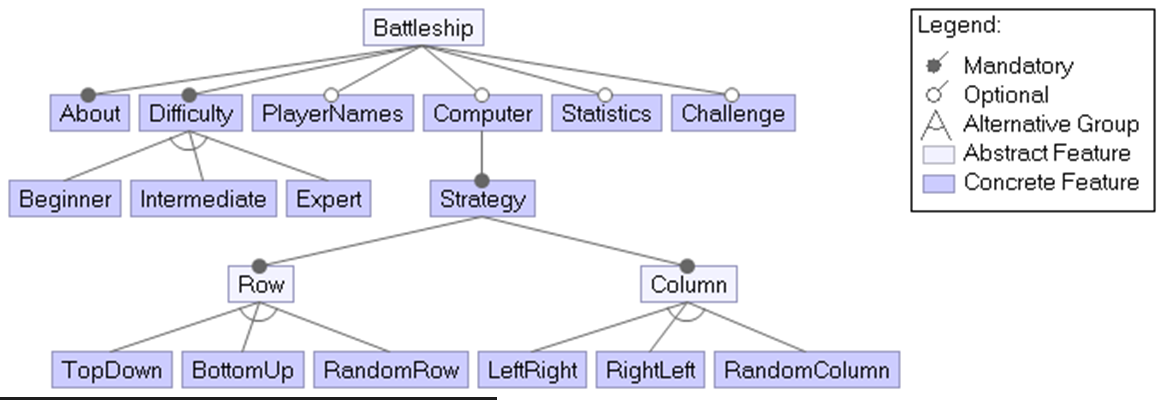
\includegraphics[width=\linewidth]{fig/battleshipFeatureModel.png}
									\caption{Feature diagram for Java Battleship game}
									\label{battleshipFeatureModel}
					\end{center}
\end{figure}


\section{Refactoring of Battleship game with using AspectJ language} \label{gameRefactoring}


\begin{figure}[t]  %vycentrovany obrazok grafu, vsadeny do odstavca
					\begin{center}
									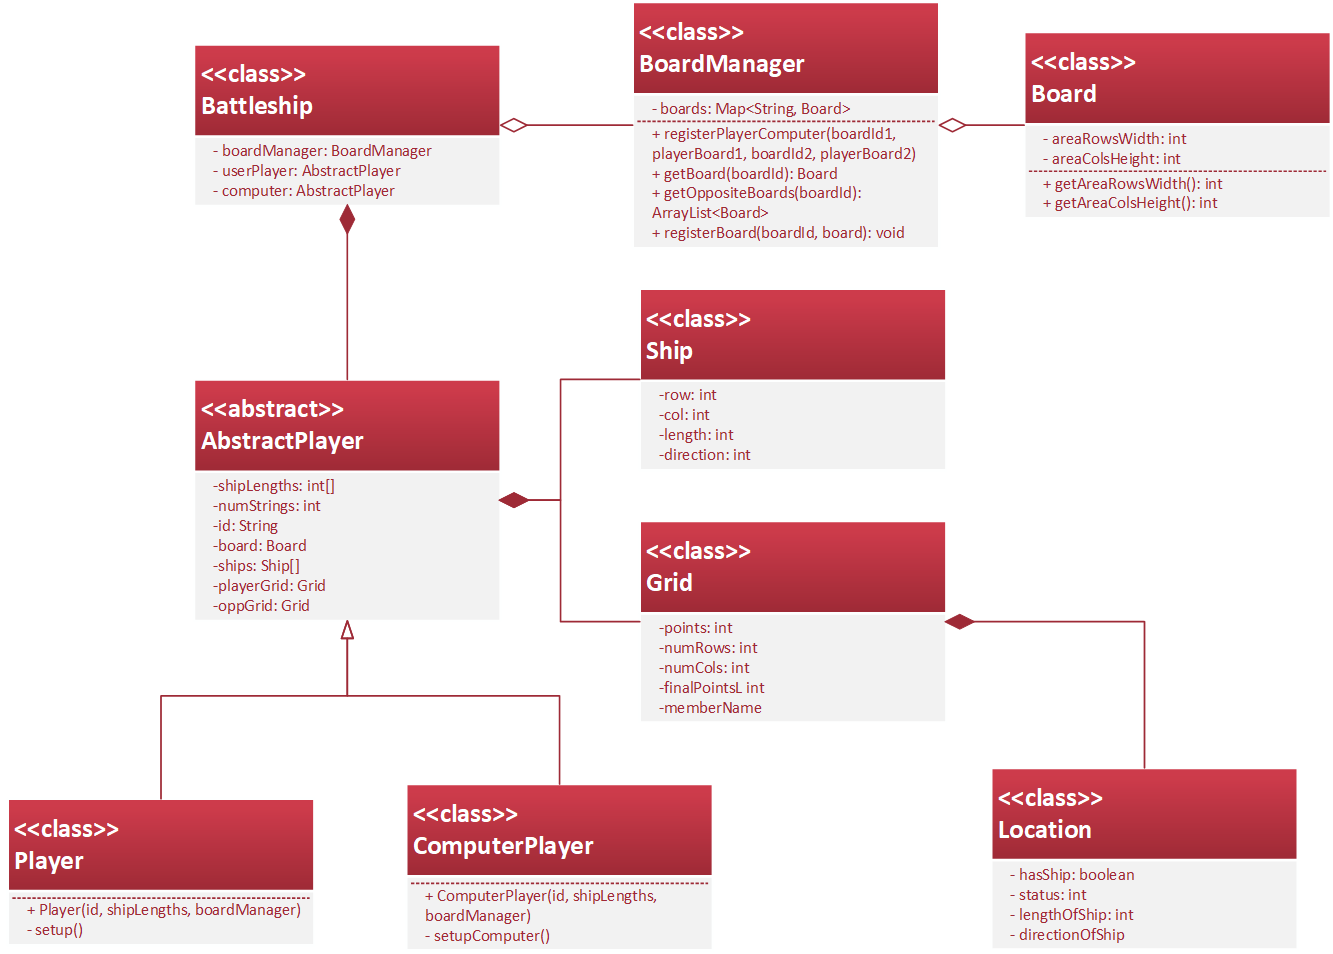
\includegraphics[width=\linewidth]{fig/refactoredSchema.png}
									\caption{Class Diagram of modified solution}
									\label{refactoredSchema}
					\end{center}
\end{figure}


\begin{figure}[H]  %vycentrovany obrazok grafu, vsadeny do odstavca
					\begin{center}
									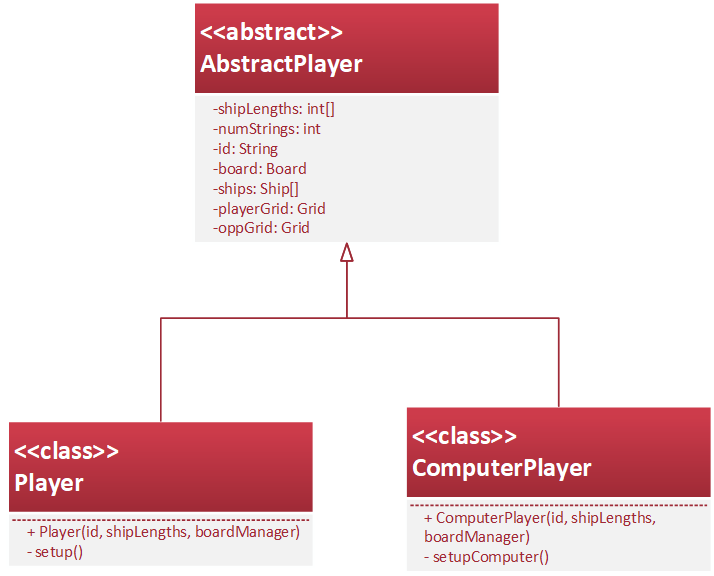
\includegraphics[height=10cm]{fig/playerAbstraction.png}
									\caption{Player abstraction}
									\label{playerAbstraction}
					\end{center}
\end{figure}

Po prvej iterácii je diagram balíkov zobrazený na obrázku \ref{problemsOfAspectJ}.

\begin{figure}[H]  %vycentrovany obrazok grafu, vsadeny do odstavca
					\begin{center}
									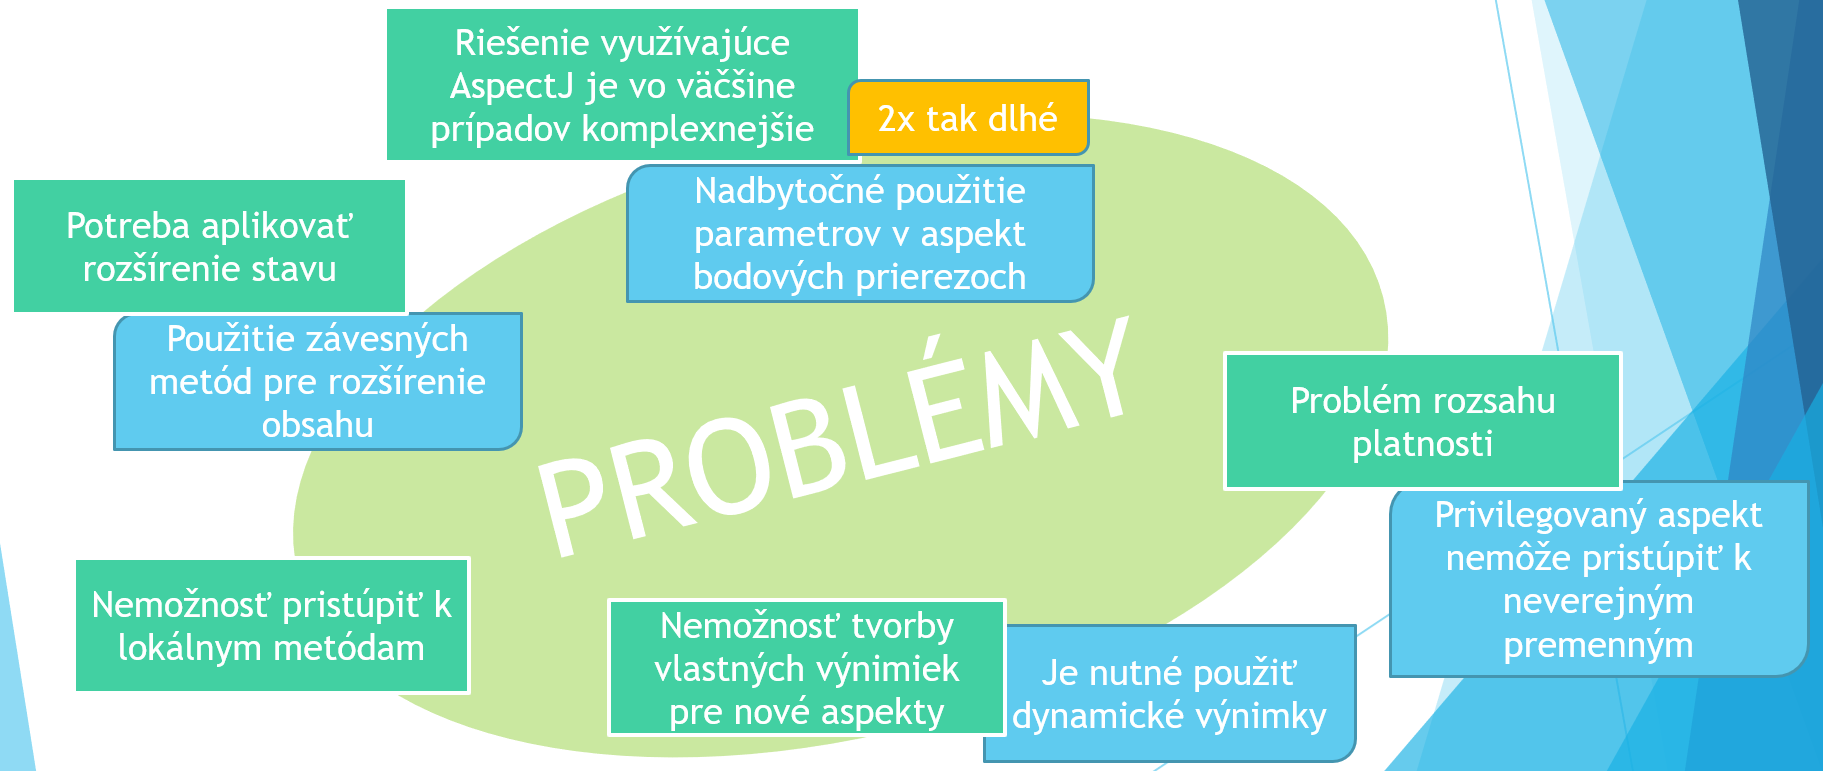
\includegraphics[width=\linewidth]{fig/problemsOfAspectJ.png}
									\caption{Problémy použitia jazyka AspectJ}
									\label{problemsOfAspectJ}
					\end{center}
\end{figure}



\section{Derivation of given Battleship game} \label{gameDerivation}

If classes and aspects are available there should be question how to separate given features from others except only configure aspects.
We come with idea, that we can copy files or part of them which represents required features. It will be based on feature models as previous part. Mandatory features from the top of the three always should be copied. Other features deeper in feature tree often require from their parents to be included. This creates new problem how to copy such files. We needed rules which can be mappped to features. We again come with idea of creating annotations with expression enabling specify condition when such feature should be copied and when not. Mapping of some features with given values to feature tree can be seen on picture \ref{derivationRules}. For example if variable playerNames is true, then it all necessary classes for this feature will be copied in final solution. If rule will be empty then will be evaluated as true. If any  file will be without annotation or all rules of its annotations will be false, then file will not be copied into final solution.

\begin{figure}[H]  %vycentrovany obrazok grafu, vsadeny do odstavca
					\begin{center}
									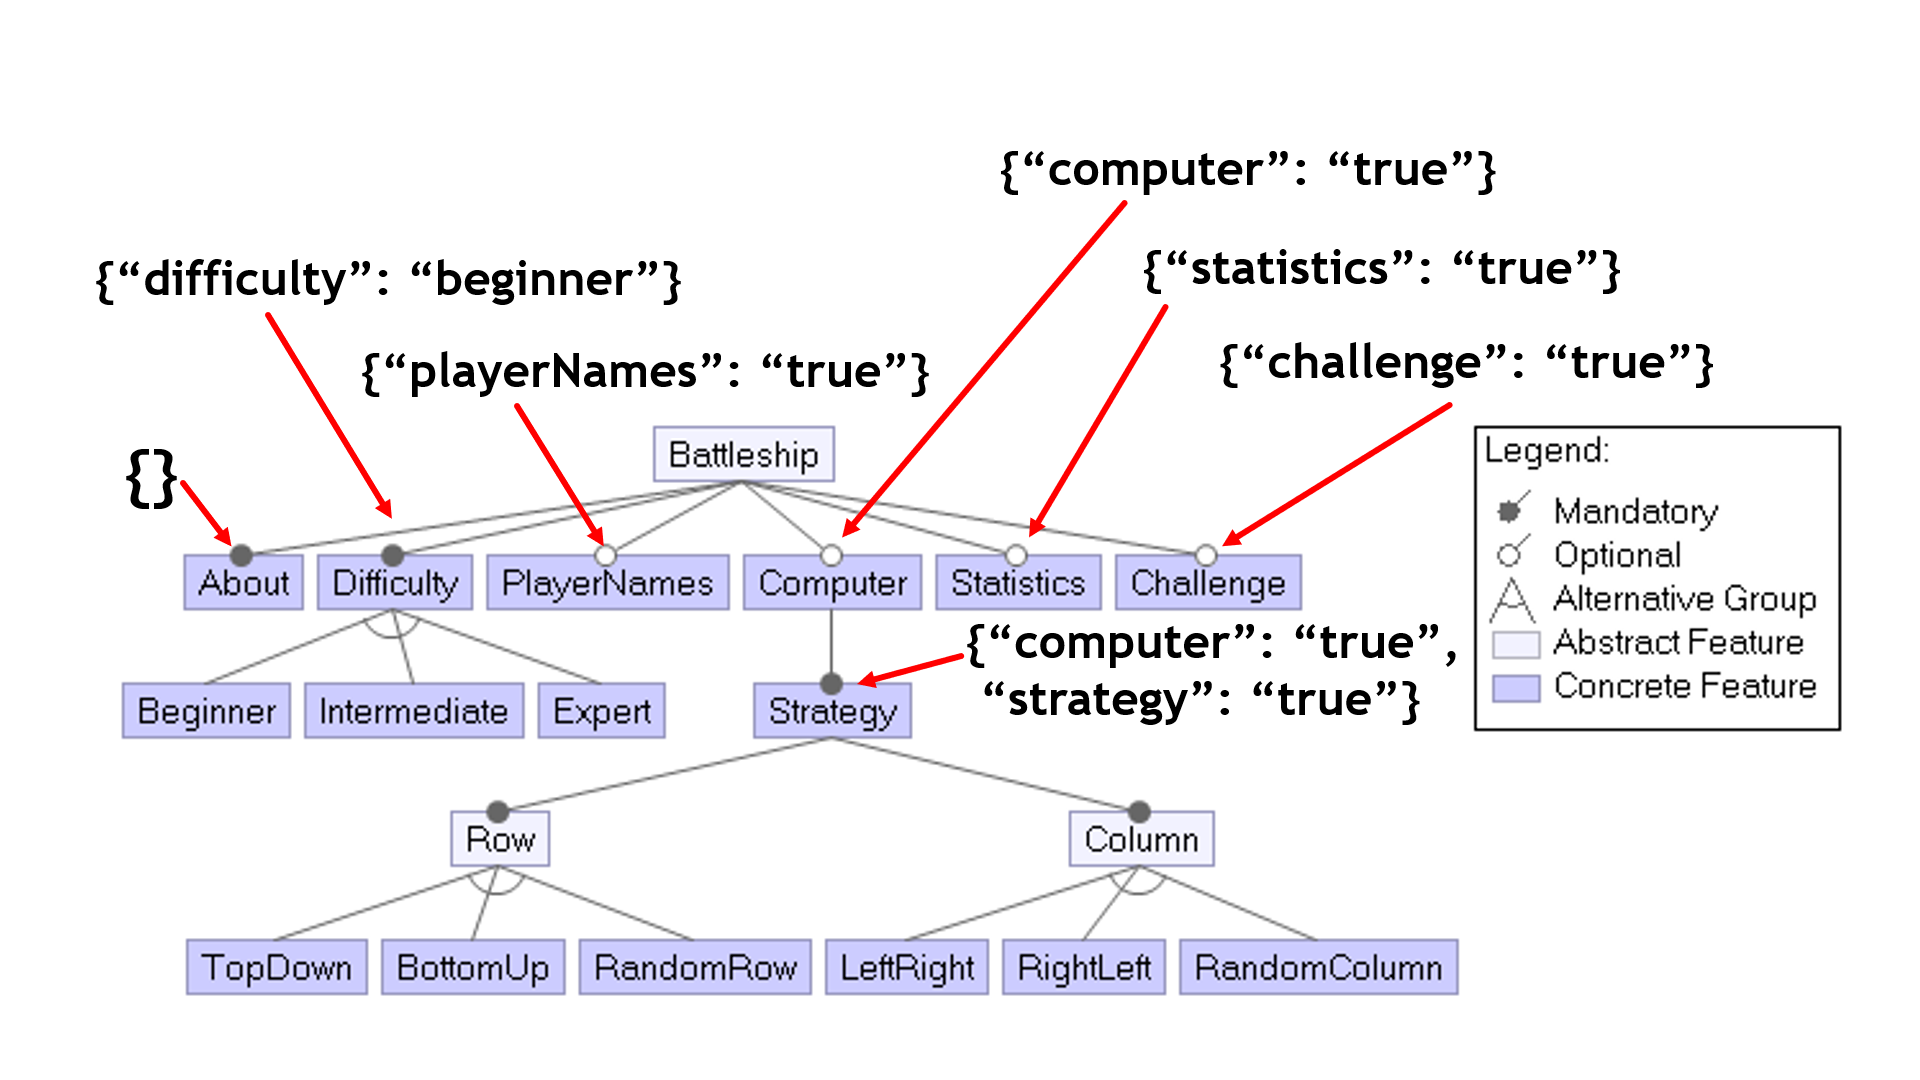
\includegraphics[width=\linewidth]{fig/derivationRules.png}
									\caption{Derivation rules}
									\label{derivationRules}
					\end{center}
\end{figure}


We specified three types of annotations:

\begin{enumerate}
	\item The first annotation is //@\{\}. This annotation can be used on classes, interfaces or aspects to copy whole file. Additional check can be added to program, that one of these keywords should be included after annotation.

	\item The second annotation is //\#\{\}. This annotation is suitable for include or exclude given methods. If file should be copied then at least one condition of annotation should be true. It should not be mixed with first one. 

	\item The third annotation is //\%\{\}. Using this annotation some imports can be included or excluded according including or excluding given method from file. It can be used with second type of annotation. 
\end{enumerate}

We mainly use first type of annotation, but in some cases remaining two should be used. Because that solution is modular it is possible to copy all files for each feature and make derived product functional. We can say so in situation where splitting some files with many features occurring at one place can be solution, but destroing such entities and their responsibilities at all. Because of it remaining two annotations are used. Content can be managed effectively then. Because we include or exclude methods and they can import classes which in some cases will not be part of final solution its necessary to annotate them using third annotation to be included or excluded. Typical example is functionality for setting names. Two methods are annotated with second annotation. Both of them expects that variable setNames will be true if they should be included. Only second method for setting computer name has another condition in annotation that computerOpponent variable should be set to true, otherwise method will not be copied. 
 
For making more complex condition we enable to use AND and OR operators to specify relation between variables as is described on picture \ref{complexDerivationRule}. We use recursion to evaluate them. If no operators are used expression is evaluated as AND statement. For AND operator all children should be true. For OR operator at least one should be true.

\begin{figure}[t]  %vycentrovany obrazok grafu, vsadeny do odstavca
					\begin{center}
									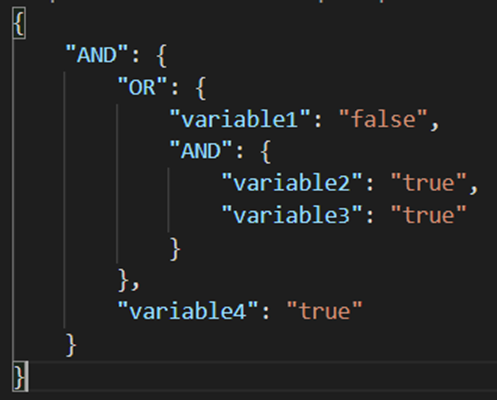
\includegraphics[width=\linewidth]{fig/expresion.png}
									\caption{Zložený derivačný výraz}
									\label{complexDerivationRule}
					\end{center}
\end{figure}

Class diagram for given solution is depicted on picture \ref{derivationProductClassDiagram}. DerivationManager class manages derivation and contain all necessary tools for this operations. For example project copier to copy empty project without classes or FileCopy class to manage reading and writing of given file as stream. During copying is necessary to find if file should be coped or not. For this purpose program needs to find annotation and evaluate its expressions. Searching is done by DerivationAnnotationManager which is using abstract class DerivationAnnotation with all of possible derivation annotation classes which extends this mentioned abstract class and deals with its own type of processing annotation. Available are methods working with StringBuilder to save string for later or Writer to write values immediately. Each annotation should check if some keywords are included. For example aspect, interface or class for first type of annotation. DerivationVariableProcessor class helps DerivationAnnotationManager to evaluate expression associated with annotation. Provided implementation should evaluate expressions with AND and OR operators too. It needs to know used variables and their values to decide mentioned expression correctly. Mapping is provided by ConfigurationVariableManager.

\begin{figure}[t]  %vycentrovany obrazok grafu, vsadeny do odstavca
					\begin{center}
									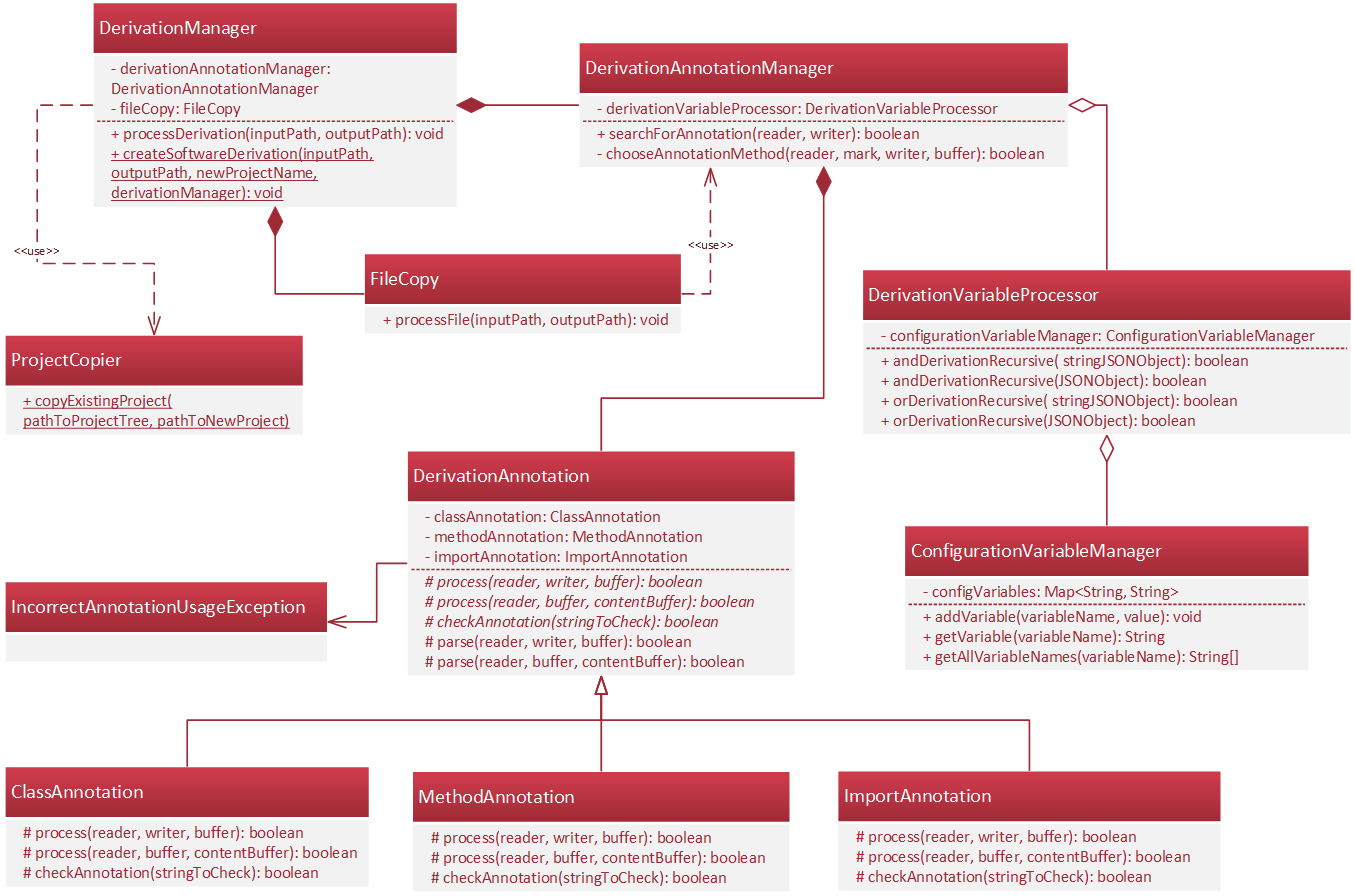
\includegraphics[width=\linewidth]{fig/DerivationClass.png}
									\caption{Class diagram for product derivation}
									\label{derivationProductClassDiagram}
					\end{center}
\end{figure}


We also model dynamic behavior for this generator as is depicted on picture \ref{derivationProductSequenceDiagram}. At the beginning developer chooses features setting values to configuration file. After method for derivation is called and configuration file is applied then DerivationManager class firstly copy empty project to specified result place. After it FileCopy class is used. For each file in source src directory tries to find annotation using DerivationAnnotationManager. If annotation is found then DerivationVariableProcessor class evaluates condition. If condition is true, annotation is processed using given implementation for given type of annotation. If file not have annotations or all expressions results in false result then the file will be deleted.

\begin{figure}[!t]  %vycentrovany obrazok grafu, vsadeny do odstavca
					\begin{center}
									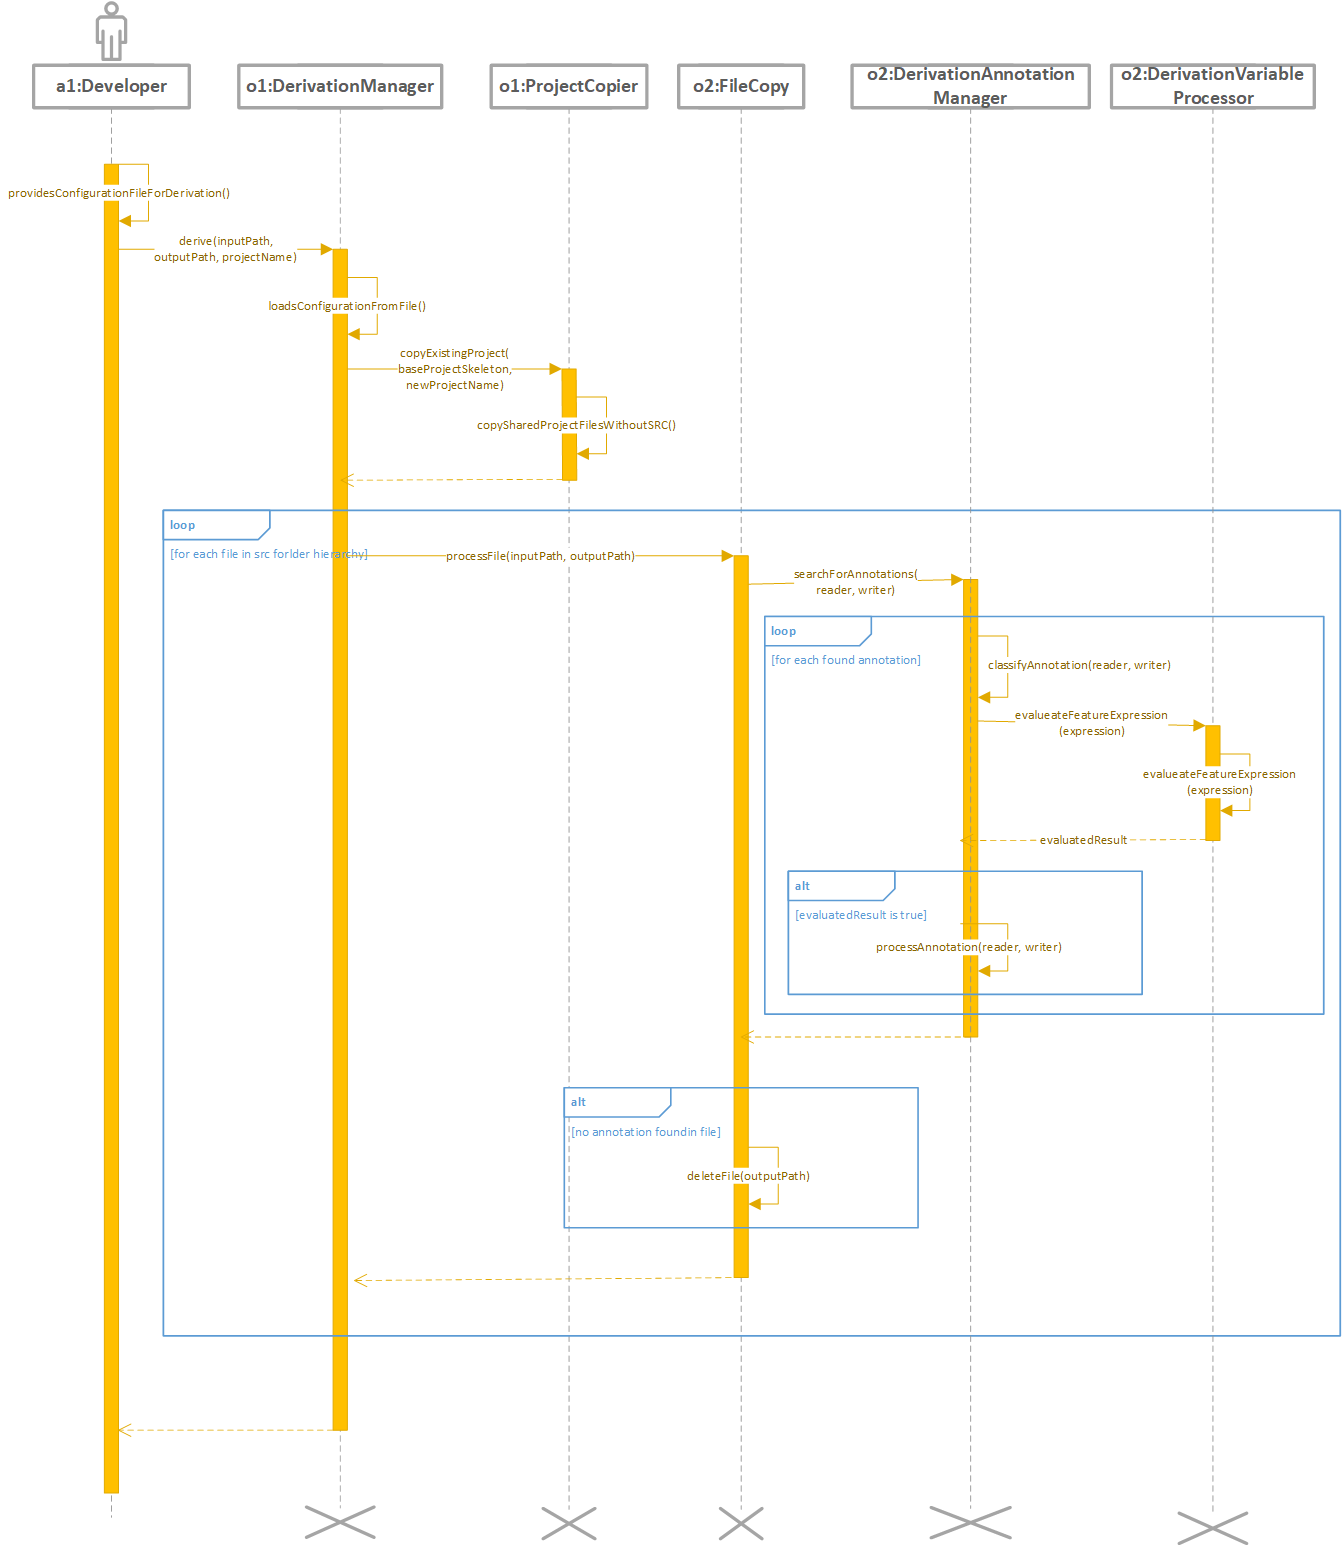
\includegraphics[width=\linewidth]{fig/derivationProcess.png}
									\caption{Sekvenčný diagram pre deriváciu produktu}
									\label{derivationProductSequenceDiagram}
					\end{center}
\end{figure}


\section{Derivation of all types of Battleship games} \label{allDerivations}

Feature models helps to determine variability in solution. According them it is possible to apply given derivation. We used variables from configuration too, but also other classes that generate all possible derivations. Changing configuration variables was necessary. We need to create another configuration file where variable names are specified with other information about them. For example variable type and number of possible cases. Variable can have boolean type and possible cases are two, true and false. if variable have string type, cases should be named explicitly in array. For example if we can include difficulty setting and include it in derivation products then possible cases will be three. Namely easy, medium and hard. We named configuration file as variableRestrictions.json. Generator will generate all cofiguration for all cases of given variables. For each configuration described derivation method will be called. In our project we created 2 * 2 * 2 * 2 * 3 = 48 derivations as depicts picture \ref{derivationBattleshipTypes}.  

\begin{figure}[H]  %vycentrovany obrazok grafu, vsadeny do odstavca
					\begin{center}
									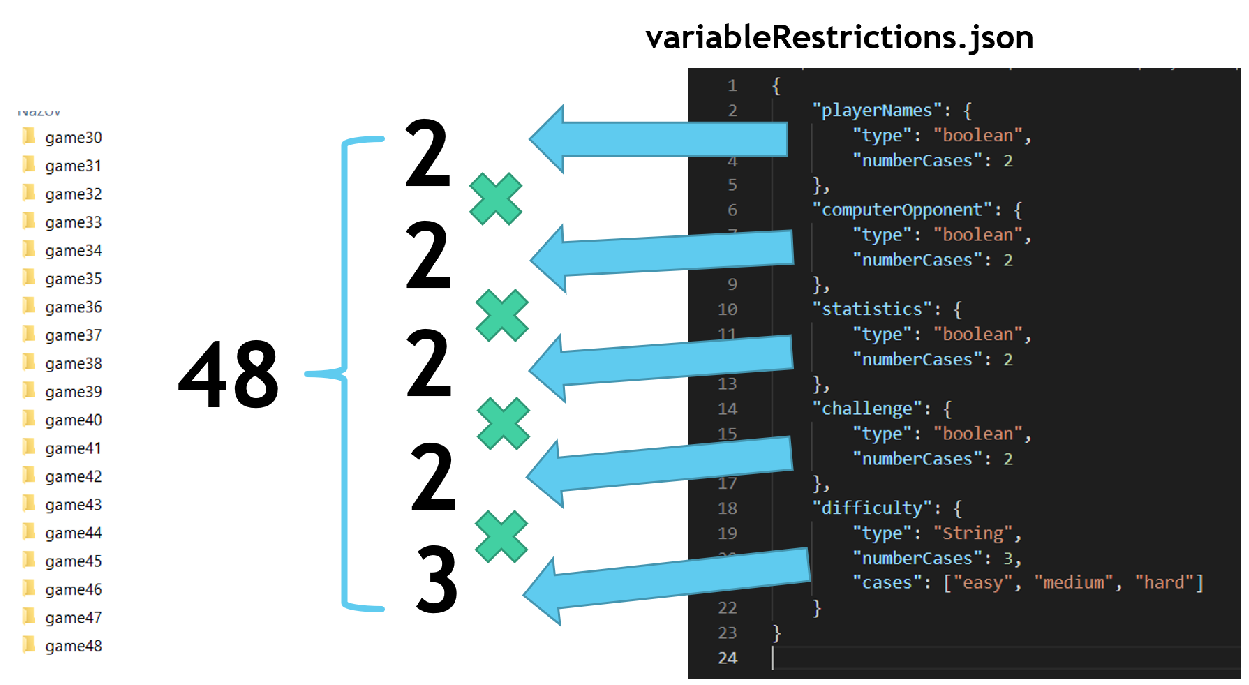
\includegraphics[width=\linewidth]{fig/allCases.png}
									\caption{Derivation of all Battleship game types}
									\label{derivationBattleshipTypes}
					\end{center}
\end{figure}


\section{Software product line for fractals} \label{fractalProductLine}

Generating fractals should be interesting application in software product line design. Not only mathematical approach, but also user requirement should be applied during development. Feature models will then vary according these requirements. To evaluate resulting shapes and use their variable basis is necessary to derive such software enabling to draw fractals. All possible derivations should be created for their aesthetic evaluation to see which of them provides value to our perception. After this phase its possible to continue with development using certain derivations and enhance their structure.

During fractals analysis we found many types of fractals. Some of them are created dividing certain shapes to some extent like Sierpinskeho fractal, others extends to space using given iteration parameter. The length of line not changes during iterations. Examples are w-curves or Krishna anklet. Some for other types are created using rotation of lines in space. For example Koch snowflake or hexagram. Mentioned algorithm type used to generate fractal can be enhanced by adding more shapes on user request. Not only parameters of algorithm will apply there. Lot of parameters are possible there. For example radius of circles, or different length of given shapes, width of the line, ommiting certain recursion calls or drawing unfilled lines as exchange for given line. With unfilled lines its possible to manage diameter between these lines. We applied given approach drawing w-curves and results shows interesting shapes apart from w-curve shape using high value for this diameter. Software product lines can help in such situations to generate all types easily and only evaluate given result when launching application is only remaining requirement.

\begin{figure}[H]  %vycentrovany obrazok grafu, vsadeny do odstavca
					\begin{center}
									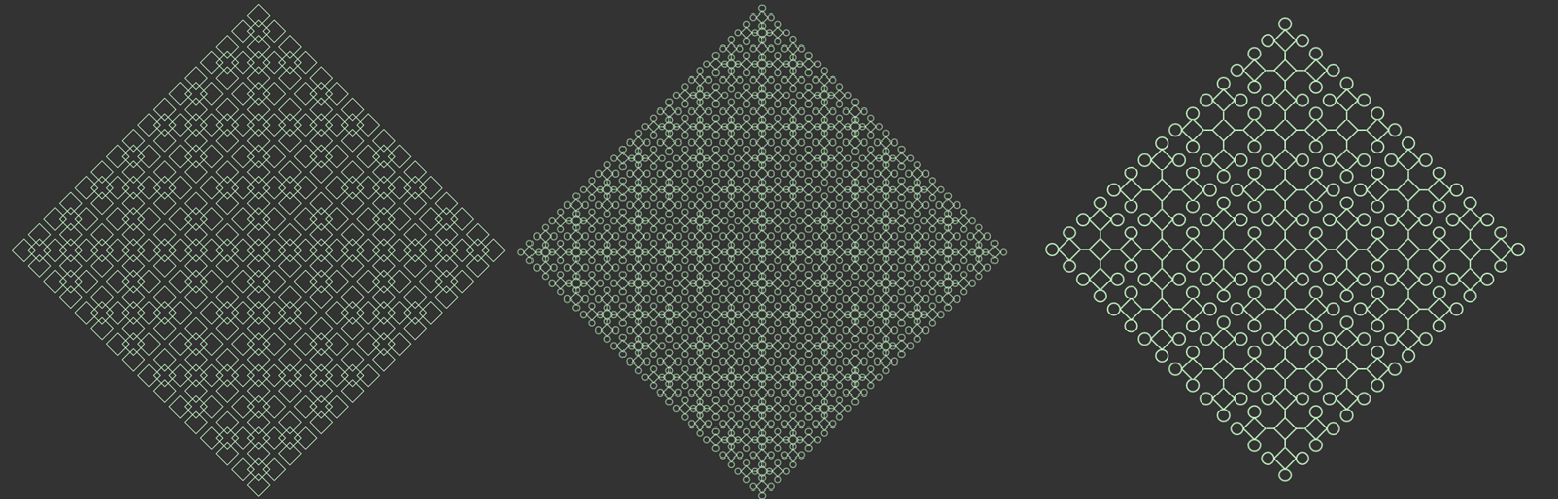
\includegraphics[width=\linewidth]{fig/fractalsAnklet.png}
									\caption{Different anklet fractal shapes}
									\label{ankletFractalTypes}
					\end{center}
\end{figure}



\section{Resulting modularity and derived products} \label{resultingModularity}

Aspect helps to produce modular solutions and enhance functionality without modifying of existing code. In case of separating concerns using them can prevent code scattering. Large parts of interacting code for logging, exception handling, third party functionality which is used because of code improvements can be moved to separated classes and let main logic for each concern remain in given place without such code directly included. Mentioned parts of such concerns are included during weaving. In case of product line approach we found that is possible to introduce mechanism to easy copy certain parts of given project and let project to be functional and possibly prepared for next development phase. 


\subsection{Modification of functionality and use of AspectJ language} \label{functionalityModiffication}

Developed game using AspectJ shows these mentioned benefits as crucial for purpose of this application. Other benefits using AspectJ enabling easier configuration provided by changing method calls with values provided by chosen approach. These approach can be changed only by adding or removing given aspects from execution. Developing such aspect requires only changing core of few methods of one type of given aspect copy to reach this goal. Aspects well suits for required features too. They well cover variable features. Adding such feature needs to prepare given aspects and join points for them. Application should be developed in respect to changing requirements. Provided code then should be parameterized because of enabling use of many features and possibility to configure application.

Using aspect not brings only benefits to development and refactoring of existing solution. AspectJ requires to include certain refactoring and code modifications to hangs certain aspects on these modified parts. Aspects pointcuts are twice as long and lot of provided parameters are repeated many times. If these pointucts are modified only in few places their copy is unreadable and is hard to distinguish amongst them. Other crucial problem is need to create empty methods called hooks to hang up certain aspect on them, because aspect oriented methods for changing behaviour of code inside method are missing. In many cases aspects are applied only on one method, not groups of methods. In larger applications it can happen that private variables are exposed to priviledged aspects and all encapsulation benefits are lost. AspectJ is not only language witch supports aspect oriented programming, but in my opinion its most powerful way for software product line development including product derivation.


\subsection{Generating derivation of Battleship game} \label{gameDerivationBattleship}

During our work we created annotations which enable selection of given classes, interfaces and aspects in final derivation. We prepared and connected these classes with configuration file to make such selection to be based on actual configuration. Changing one variable results in applied derivation and creation of different result. We let to generate all possible derivations for all implemented variable features from feature model to prove its functionality. We need only three type of basic annotations to mark classes to separate them. We also developed algorithm to evaluate expression which enables copy given files to result project. Expression consists of variables which identifies features of given feature model which serves as basis for software product line application.    


\section{Recent work} \label{recentWork}

Kód kt


\section{Conclusions and next work} \label{conclusions}

Analyzo
 

\bibliographystyle{abbrv} % plain or alpha are fine, too
\bibliography{bib}


\end{document}

